% Options for packages loaded elsewhere
\PassOptionsToPackage{unicode}{hyperref}
\PassOptionsToPackage{hyphens}{url}
\documentclass[
  ignorenonframetext,
  aspectratio=169,
]{beamer}
\newif\ifbibliography
\usepackage{pgfpages}
\setbeamertemplate{caption}[numbered]
\setbeamertemplate{caption label separator}{: }
\setbeamercolor{caption name}{fg=normal text.fg}
\beamertemplatenavigationsymbolsempty
% remove section numbering
\setbeamertemplate{part page}{
  \centering
  \begin{beamercolorbox}[sep=16pt,center]{part title}
    \usebeamerfont{part title}\insertpart\par
  \end{beamercolorbox}
}
\setbeamertemplate{section page}{
  \centering
  \begin{beamercolorbox}[sep=12pt,center]{section title}
    \usebeamerfont{section title}\insertsection\par
  \end{beamercolorbox}
}
\setbeamertemplate{subsection page}{
  \centering
  \begin{beamercolorbox}[sep=8pt,center]{subsection title}
    \usebeamerfont{subsection title}\insertsubsection\par
  \end{beamercolorbox}
}
% Prevent slide breaks in the middle of a paragraph
\widowpenalties 1 10000
\raggedbottom
\AtBeginPart{
  \frame{\partpage}
}
\AtBeginSection{
  \ifbibliography
  \else
    \frame{\sectionpage}
  \fi
}
\AtBeginSubsection{
  \frame{\subsectionpage}
}
\usepackage{iftex}
\ifPDFTeX
  \usepackage[T1]{fontenc}
  \usepackage[utf8]{inputenc}
  \usepackage{textcomp} % provide euro and other symbols
\else % if luatex or xetex
  \usepackage{unicode-math} % this also loads fontspec
  \defaultfontfeatures{Scale=MatchLowercase}
  \defaultfontfeatures[\rmfamily]{Ligatures=TeX,Scale=1}
\fi
\usepackage{lmodern}
\ifPDFTeX\else
  % xetex/luatex font selection
\fi
% Use upquote if available, for straight quotes in verbatim environments
\IfFileExists{upquote.sty}{\usepackage{upquote}}{}
\IfFileExists{microtype.sty}{% use microtype if available
  \usepackage[]{microtype}
  \UseMicrotypeSet[protrusion]{basicmath} % disable protrusion for tt fonts
}{}
\makeatletter
\@ifundefined{KOMAClassName}{% if non-KOMA class
  \IfFileExists{parskip.sty}{%
    \usepackage{parskip}
  }{% else
    \setlength{\parindent}{0pt}
    \setlength{\parskip}{6pt plus 2pt minus 1pt}}
}{% if KOMA class
  \KOMAoptions{parskip=half}}
\makeatother
\usepackage{longtable,booktabs,array}
\usepackage{caption}
\captionsetup[table]{skip=6pt}
\newcounter{none} % for unnumbered tables
\usepackage{calc} % for calculating minipage widths
\usepackage{caption}
% Make caption package work with longtable
\makeatletter
\def\fnum@table{\tablename~\thetable}
\makeatother
\usepackage{graphicx}
\makeatletter
\newsavebox\pandoc@box
\newcommand*\pandocbounded[1]{% scales image to fit in text height/width
  \sbox\pandoc@box{#1}%
  \Gscale@div\@tempa{\textheight}{\dimexpr\ht\pandoc@box+\dp\pandoc@box\relax}%
  \Gscale@div\@tempb{\linewidth}{\wd\pandoc@box}%
  \ifdim\@tempb\p@<\@tempa\p@\let\@tempa\@tempb\fi% select the smaller of both
  \ifdim\@tempa\p@<\p@\scalebox{\@tempa}{\usebox\pandoc@box}%
  \else\usebox{\pandoc@box}%
  \fi%
}
% Set default figure placement to htbp
\def\fps@figure{htbp}
\makeatother
\setlength{\emergencystretch}{3em} % prevent overfull lines
\providecommand{\tightlist}{%
  \setlength{\itemsep}{0pt}\setlength{\parskip}{0pt}}
% Auto-generated by infrastructure/rendering/_pdf_latex_helpers.py::extract_math_font_preamble.
% Minimal header passed to Pandoc via -H so Beamer slides pick up the same math font
% as the combined-PDF path. Adjust the manuscript's preamble.md to change the font globally.
\usepackage{unicode-math}
\setmathfont{latinmodern-math.otf}

% Manuscript macro/package fallbacks (newcommand -> providecommand).
% Core mathematics
\usepackage{amsmath}
\usepackage{amssymb}
% Document layout
% Tables
\usepackage{booktabs}
% Caption styling (booktabs already loaded above). Small caption font with a
% bold label ("Figure 1", "Table 2") gives the math/figure-heavy layout a
% consistent, journal-like caption rhythm without fighting pandoc-crossref —
% pandoc emits standard \caption{}, and caption/captionsetup only restyle it.
% ── Theorem environments ─────────────────────────────────────────────────
% amsthm is loaded above. The FedGVI<->Friston bridge is stated as a small
% number of theorems/definitions/lemmas/propositions/corollaries; sharing one
% counter (definition/lemma/proposition/corollary all step the `theorem`
% counter) gives a single monotone numbering 1, 2, 3, ... across all kinds, so
% authors can reference them as Theorem 1, Definition 2, Corollary 3 without a
% per-kind counter drifting out of order. Plain style for theorem-like results,
% definition style (upright body) for definitions.
% (algorithm2e intentionally not loaded: this manuscript states results as
% numbered amsthm Theorems/Definitions, not algorithm2e pseudocode.)
% Code listings
\usepackage{listings}
% Typography and formatting
% (siunitx intentionally not loaded: no \SI/\num units appear in this manuscript.)
% Cross-references and citations
% (cleveref and titlesec intentionally not loaded: unavailable in this TeX tree
% and not required. Cross-references resolve through pandoc-crossref's own
% \ref-style names — no \cref appears — and section heading styling falls back
% to the pandoc/LaTeX defaults.)
% ── TeX Live Basic-compatible mono font for code listings ────────────
% Latin Modern Mono is bundled with TeX Live Basic and keeps the manuscript
% renderable on minimal TeX installations. Mathematical Unicode coverage is
% provided separately by Latin Modern Math below, so the code font does not
% need a private JuliaMono installation.
%
% Use the TeX font filename rather than the system-family name: the minimal
% TeX Live fontconfig database may not register the OpenType family even though
% kpsewhich can resolve the bundled files.
% Math font for unicode-math: Latin Modern Math (TeX Live) has full BMP
% coverage including U+2223 (\mid), U+226A/226B (\ll/\gg), and the Greek/
% blackboard letters used in equations. Without an explicit \setmathfont,
% unicode-math falls back to lmroman text font which lacks several glyphs
% and emits "Missing character" warnings on every \mid in math mode.

% Slide layout defaults for warning-clean scientific decks.
\usepackage{etoolbox}
\IfFileExists{xurl.sty}{\usepackage{xurl}}{}
\IfFileExists{seqsplit.sty}{\usepackage{seqsplit}}{\newcommand{\seqsplit}[1]{#1}}
\protected\def\breakseq#1{\seqsplit{#1}}
\protected\def\breaktt#1{\begingroup\ttfamily\seqsplit{#1}\endgroup}
\setlength{\emergencystretch}{6em}
\tolerance=5000
\hbadness=10000
\hfuzz=1pt
\setlength{\tabcolsep}{2pt}
\AtBeginEnvironment{longtable}{\tiny\renewcommand{\arraystretch}{0.86}\setlength{\tabcolsep}{1pt}}
\AtBeginEnvironment{tabular}{\tiny\renewcommand{\arraystretch}{0.86}\setlength{\tabcolsep}{1pt}}
\AtBeginEnvironment{equation}{\tiny}
\AtBeginEnvironment{equation*}{\tiny}
\AtBeginEnvironment{align}{\tiny}
\AtBeginEnvironment{align*}{\tiny}
\AtBeginEnvironment{itemize}{\footnotesize}
\AtBeginEnvironment{enumerate}{\footnotesize}
\AtBeginEnvironment{description}{\footnotesize}
\setbeamerfont{caption}{size=\tiny}
\setbeamerfont{caption name}{size=\tiny}
\setbeamerfont{normal text}{size=\small}
\setbeamerfont{frametitle}{size=\small}
\setbeamerfont{section title}{size=\footnotesize}
\setbeamerfont{subsection title}{size=\footnotesize}
\setbeamertemplate{section page}{%
  \centering
  \begin{beamercolorbox}[sep=12pt,center,wd=\paperwidth]{section title}
    \parbox{0.86\paperwidth}{\centering\usebeamerfont{section title}\insertsection\par}
  \end{beamercolorbox}
}
\setbeamertemplate{subsection page}{%
  \centering
  \begin{beamercolorbox}[sep=8pt,center,wd=\paperwidth]{subsection title}
    \parbox{0.86\paperwidth}{\centering\usebeamerfont{subsection title}\insertsubsection\par}
  \end{beamercolorbox}
}
\setlength{\abovecaptionskip}{2pt}
\setlength{\belowcaptionskip}{0pt}

% Natbib and cross-reference fallbacks — slides don't load natbib
% or cleveref, but combined-PDF manuscript prose may emit these
% commands. The fallback renders citations as a bracketed key list
% and cross-references as detokenized labels so slides don't fail on
% undefined control sequences or raw underscores. \providecommand is
% a no-op if packages load later.
\providecommand{\citep}[1]{[#1]}
\providecommand{\citet}[1]{#1}
\providecommand{\citealp}[1]{#1}
\providecommand{\citeauthor}[1]{#1}
\providecommand{\citeyear}[1]{#1}
\providecommand{\cref}[1]{\texttt{\detokenize{#1}}}
\providecommand{\Cref}[1]{\texttt{\detokenize{#1}}}
\providecommand{\crefrange}[2]{\texttt{\detokenize{#1}}--\texttt{\detokenize{#2}}}
\providecommand{\Crefrange}[2]{\texttt{\detokenize{#1}}--\texttt{\detokenize{#2}}}
\providecommand{\paragraph}[1]{\textbf{#1}\ }

% Opt-in accessible presentation profile.
\setbeamerfont{normal text}{size*={20pt}{24pt}}
\setbeamerfont{frametitle}{size*={28pt}{32pt}}
\setbeamerfont{section title}{size*={28pt}{32pt}}
\setbeamerfont{subsection title}{size*={28pt}{32pt}}
\setbeamerfont{caption}{size*={16pt}{19pt}}
\setbeamerfont{caption name}{size*={16pt}{19pt}}
\setbeamerfont{itemize/enumerate body}{size*={20pt}{24pt}}
\setbeamerfont{itemize/enumerate subbody}{size*={20pt}{24pt}}
\setbeamerfont{itemize/enumerate subsubbody}{size*={20pt}{24pt}}
\setbeamerfont{itemize item}{size*={20pt}{24pt}}
\setbeamerfont{itemize subitem}{size*={20pt}{24pt}}
\setbeamerfont{itemize subsubitem}{size*={20pt}{24pt}}
\setbeamerfont{description body}{size*={20pt}{24pt}}
\setbeamerfont{description item}{size*={20pt}{24pt}}
\setbeamerfont{quote}{size*={20pt}{24pt}}
\setbeamerfont{quotation}{size*={20pt}{24pt}}
\AtBeginEnvironment{longtable}{\fontsize{20pt}{24pt}\selectfont}
\AtBeginEnvironment{tabular}{\fontsize{20pt}{24pt}\selectfont}
\AtBeginEnvironment{equation}{\fontsize{20pt}{24pt}\selectfont}
\AtBeginEnvironment{equation*}{\fontsize{20pt}{24pt}\selectfont}
\AtBeginEnvironment{align}{\fontsize{20pt}{24pt}\selectfont}
\AtBeginEnvironment{align*}{\fontsize{20pt}{24pt}\selectfont}
\AtBeginEnvironment{itemize}{\fontsize{20pt}{24pt}\selectfont}
\AtBeginEnvironment{enumerate}{\fontsize{20pt}{24pt}\selectfont}
\AtBeginEnvironment{description}{\fontsize{20pt}{24pt}\selectfont}
\AtBeginDocument{\usebeamerfont{normal text}}
\newlength{\AFSlideTableWidth}
% The fixed footer reservation is calibrated with the semantic seven-line regular-body budget.
\setbeamertemplate{footline}{%
  \leavevmode\vbox{%
    \hbox{%
      \begin{beamercolorbox}[wd=\paperwidth,ht=16pt,dp=3pt,center]{author in head/foot}%
        \fontsize{16pt}{19pt}\selectfont Untagged PDF derivative \textbar\ \href{../web/index.html}{HTML reader}%
      \end{beamercolorbox}%
    }%
    \vskip6pt%
  }%
}
% Accessible footer reserved height: 25pt.

\newtheorem{proposition}{Proposition}
\newtheorem{hypothesis}{Hypothesis}
\newtheorem{remark}[theorem]{Remark}
\newtheorem{axiom}{Axiom}
\newtheorem{property}{Property}
\usepackage{bookmark}
\IfFileExists{xurl.sty}{\usepackage{xurl}}{} % add URL line breaks if available
\urlstyle{same}
% fallback for those not using the hyperref driver hyperxmp:
\makeatletter
\@ifundefined{xmpquote}{\newcommand{\xmpquote}[1]{#1}}{}
\makeatother
\hypersetup{
  hidelinks,
  pdfcreator={LaTeX via pandoc}}

\author{\texorpdfstring{}{}}
\date{}

\begin{document}

\section{Reproducibility: execution record and application
integrity}\label{sec:reproducibility}

\begin{frame}{Reproducibility: execution record and application
integrity}
This section is a machine-verifiable reproducibility certificate. Every
value below is computed by the analysis pipeline and injected at render
time, establishing a chain of custody from configuration through code to
publication.
\end{frame}

\begin{frame}{Reproducibility (part 2)}
The discipline is the one that gates this project's CI: every prose
number is a generated token, every token is emitted by one generator
function,
\end{frame}

\begin{frame}{Reproducibility (part 3)}
and any drift between narrative and computed result fails the build
before a green PDF exists (Peng 2011).
\end{frame}

\begin{frame}{Determinism contract for seeded scientific results}
\protect\phantomsection\label{sec:repro-determinism}
Reproducing every reported number requires only two recorded inputs: the
global seed pinned here and the software environment fingerprinted in
the next subsection. The determinism contract fixes the first ---
\end{frame}

\begin{frame}[fragile]{Determinism contract for\ldots{} (part 2)}
it states exactly what is held constant, what is asserted to machine
tolerance, and what is deliberately not claimed byte-identical.

\textbf{Seed.} The global seed is 0, threaded through every
\texttt{np.random.default\_rng(seed)}; the global \texttt{np.random}
state is never used.
\end{frame}

\begin{frame}{Determinism contract for\ldots{} (part 3)}
\textbf{Assertions.} Recovery identities use exact or machine-tolerance
assertions; seeded study reports are regression-tested for repeatability
under the recorded software environment.
\end{frame}

\begin{frame}{Determinism contract for\ldots{} (part 4)}
Rendered PDF/HTML/slide containers are validated as fresh publication
products but are not claimed byte-identical across toolchain versions.
\end{frame}

\begin{frame}{Determinism contract for\ldots{} (part 5)}
\textbf{Execution.} No mocks are used: every test is a genuine
computation on small categorical distributions or a seeded simulation
under this repository's explicit no-mocks policy.
\end{frame}

\begin{frame}{Application integrity and solver-health receipts}
\protect\phantomsection\label{sec:repro-application-integrity}
The labeled own-data path produces a different evidentiary object from a
research report. It validates one-dimensional categorical inputs, hashes
the canonical semantic request,
\end{frame}

\begin{frame}{Application integrity and\ldots{} (part 2)}
delegates once to the shared aggregation domain, and records numerical
health without adding a decision or interpretation.
\end{frame}

\begin{frame}[fragile]{Application integrity and\ldots{} (part 3)}
The application flow in fig.~19 reads
from top to bottom. Panel A follows validation and canonical hashing;
Panel B places the exact two-by-two \texttt{solver\_status} key below
the result classifier; Panel C separates the upper atomic-write row from
the lower verification lane.
\end{frame}

\begin{frame}{Application integrity and\ldots{} (part 4)}
Invalid inputs or unsafe destinations fail before directory creation.
Non-nominal numerical results retain their artifacts and return a
distinct status rather than being silently promoted or discarded.
\end{frame}

\begin{frame}{Application integrity and\ldots{} (part 5)}
An application receipt can verify artifact integrity and, when requested
and available, source equivalence. Requiring nominal solver health adds
a numerical gate. None of those levels establishes calibration, domain
suitability, scientific validity, decision correctness, or acceptance.
\end{frame}

\begin{frame}{Application integrity and\ldots{} (part 6)}
\begin{figure}
\centering
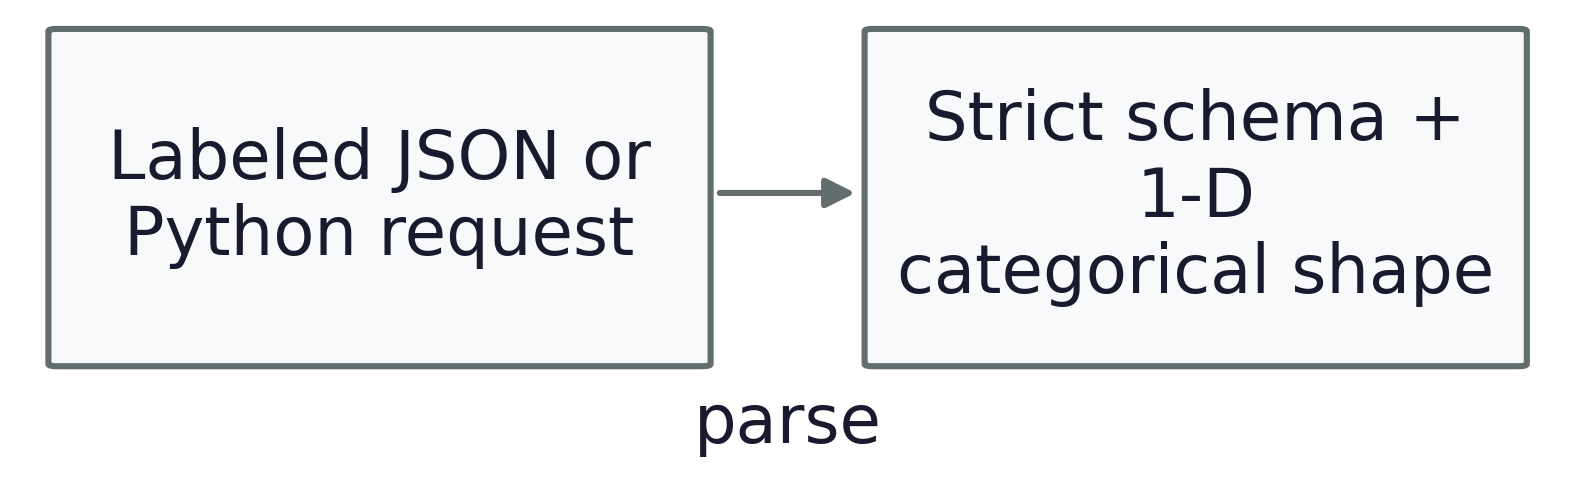
\includegraphics[keepaspectratio,width=0.98\linewidth,height=0.8\textheight,alt={Labeled JSON or Python request → Strict schema + 1-D categorical shape: parse; normal.}]{../figures/application_integrity_flow.slide-request-strict-validation.png}
\refstepcounter{figure}\label{fig:application-integrity-flow-slide-panel-1}
\end{figure}
\end{frame}

\begin{frame}{Application integrity and\ldots{} (part 7)}
\begin{figure}
\centering
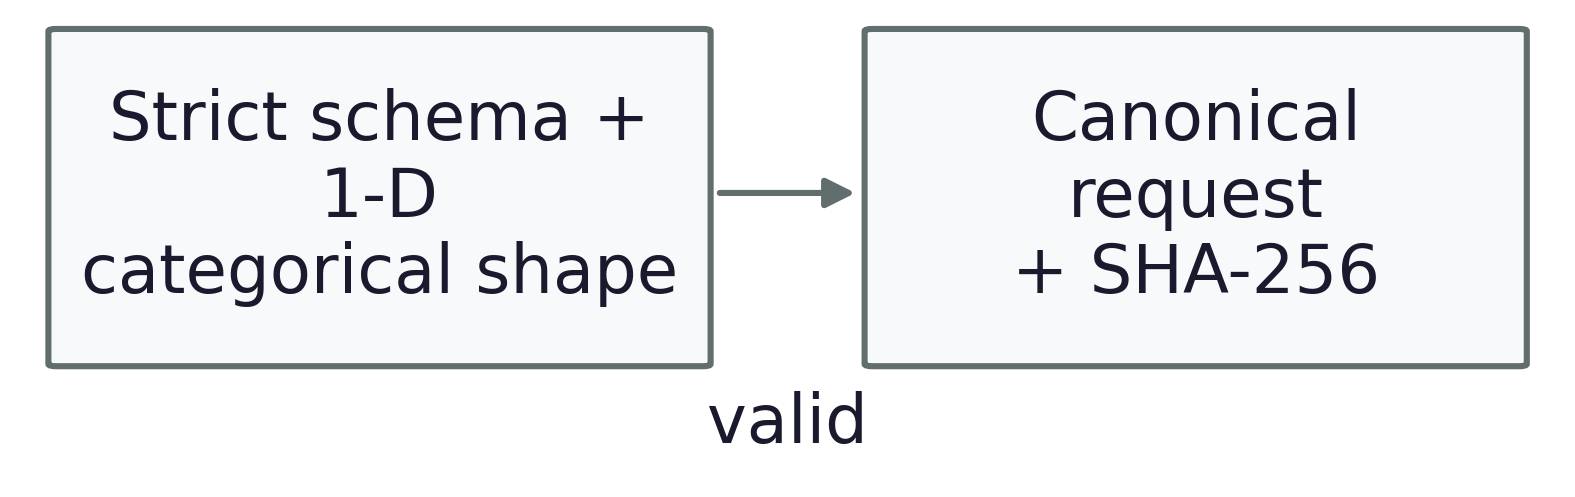
\includegraphics[keepaspectratio,width=0.98\linewidth,height=0.8\textheight,alt={Strict schema + 1-D categorical shape → Canonical request + SHA-256: valid; normal.}]{../figures/application_integrity_flow.slide-strict-validation-canonical-request.png}
\refstepcounter{figure}\label{fig:application-integrity-flow-slide-panel-2}
\end{figure}
\end{frame}

\begin{frame}{Application integrity and\ldots{} (part 8)}
\begin{figure}
\centering
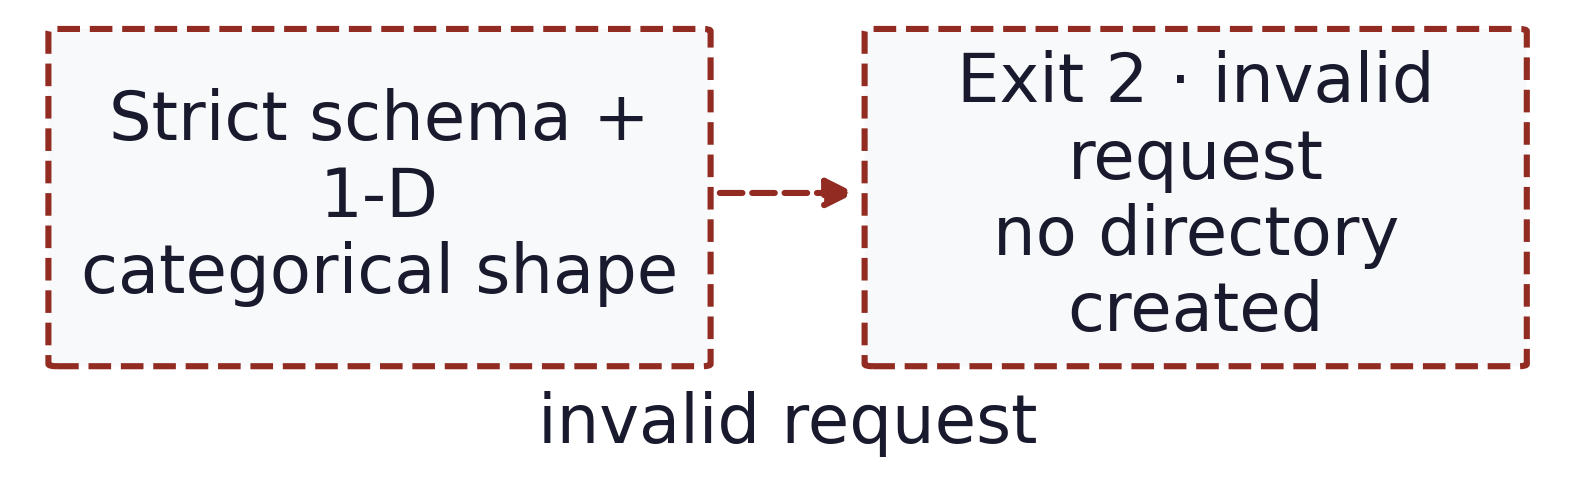
\includegraphics[keepaspectratio,width=0.98\linewidth,height=0.8\textheight,alt={Strict schema + 1-D categorical shape → Exit 2 · invalid request no directory created: invalid request; rejected.}]{../figures/application_integrity_flow.slide-strict-validation-invalid-request.png}
\refstepcounter{figure}\label{fig:application-integrity-flow-slide-panel-3}
\end{figure}
\end{frame}

\begin{frame}{Application integrity and\ldots{} (part 9)}
\begin{figure}
\centering
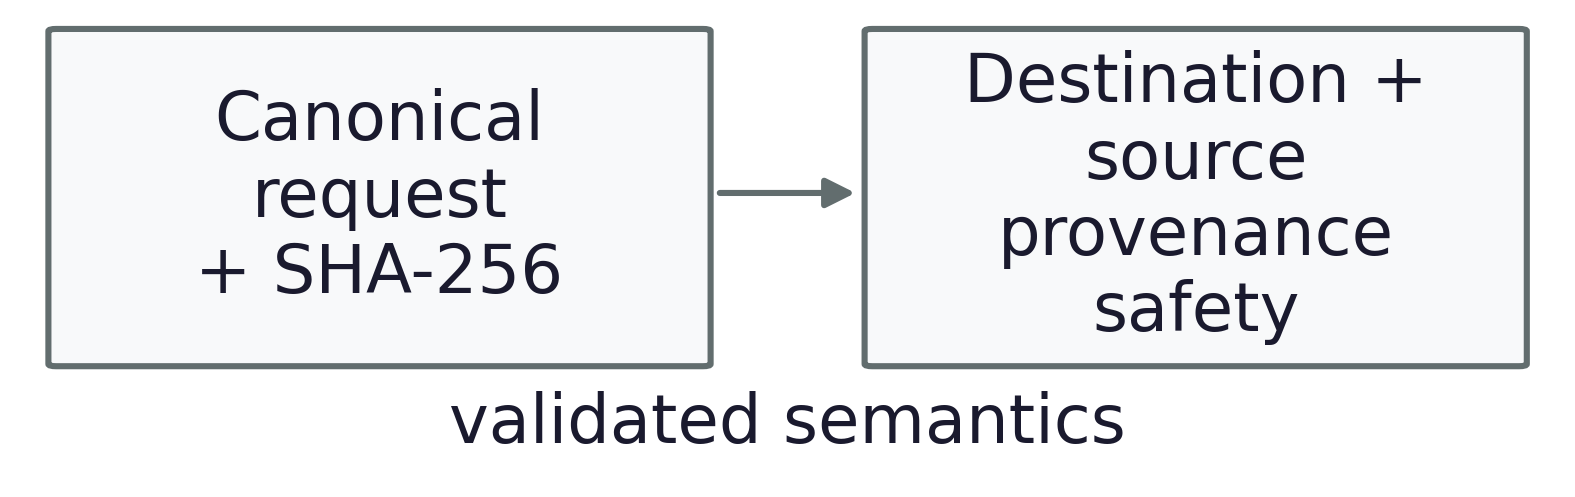
\includegraphics[keepaspectratio,width=0.98\linewidth,height=0.8\textheight,alt={Canonical request + SHA-256 → Destination + source provenance safety: validated semantics; normal.}]{../figures/application_integrity_flow.slide-canonical-request-destination-safety.png}
\refstepcounter{figure}\label{fig:application-integrity-flow-slide-panel-4}
\end{figure}
\end{frame}

\begin{frame}{Application integrity and\ldots{} (part 10)}
\begin{figure}
\centering
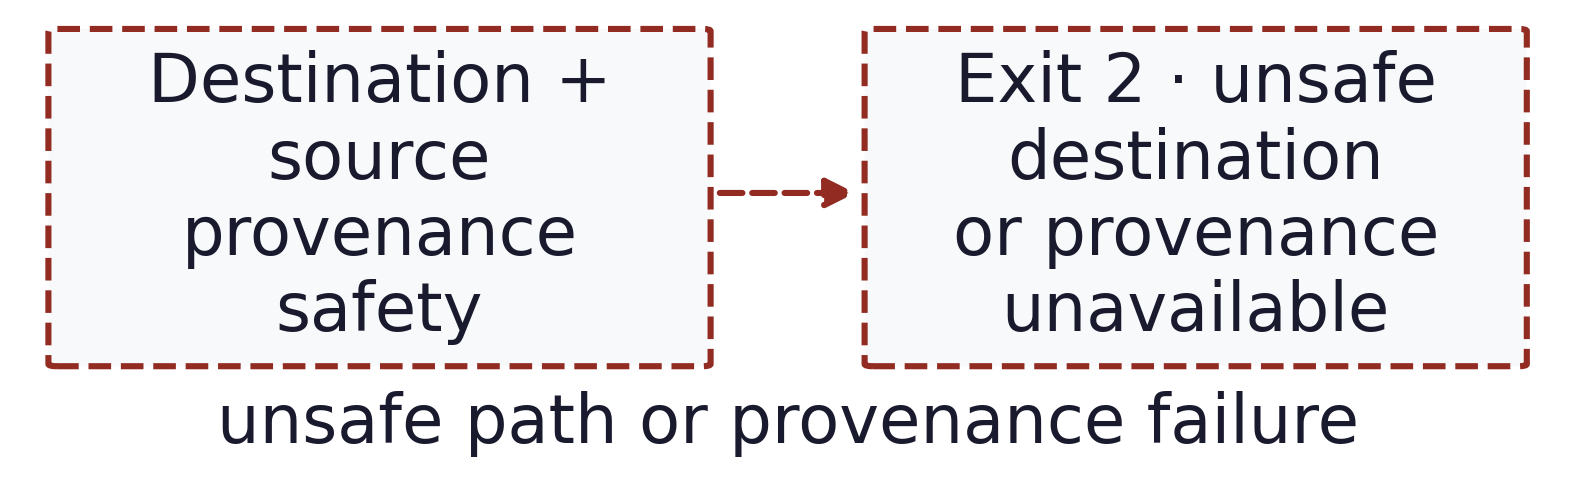
\includegraphics[keepaspectratio,width=0.98\linewidth,height=0.8\textheight,alt={Destination + source provenance safety → Exit 2 · unsafe destination or provenance unavailable: unsafe path or provenance failure; rejected.}]{../figures/application_integrity_flow.slide-destination-safety-unsafe-destination.png}
\refstepcounter{figure}\label{fig:application-integrity-flow-slide-panel-5}
\end{figure}
\end{frame}

\begin{frame}{Application integrity and\ldots{} (part 11)}
\begin{figure}
\centering
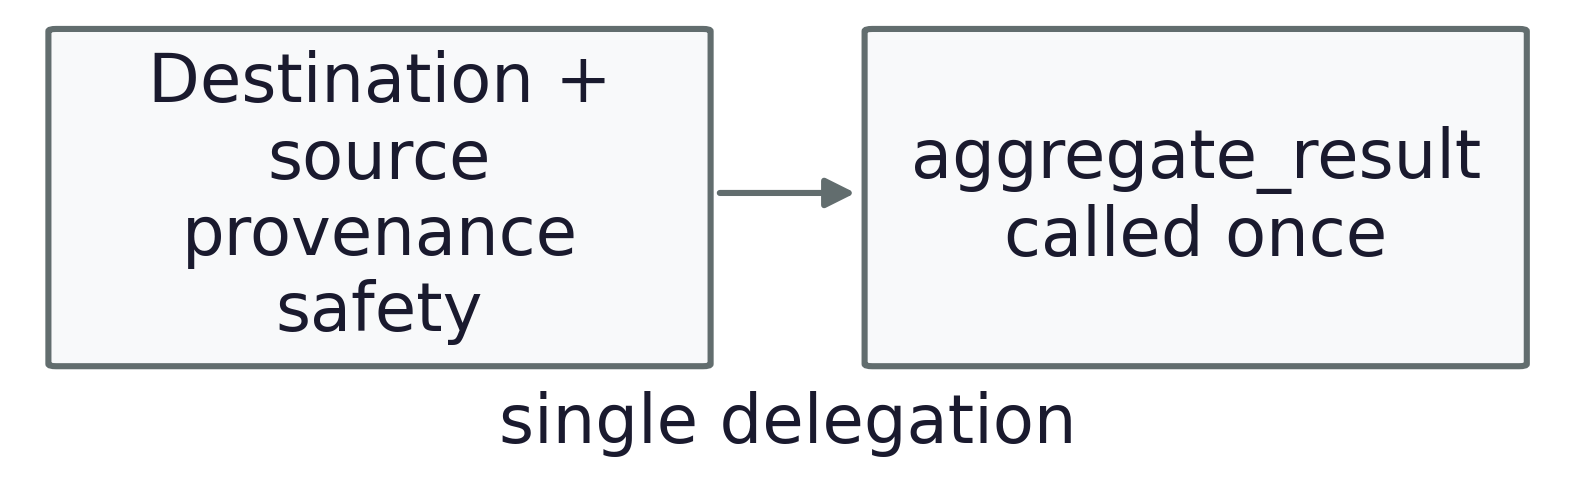
\includegraphics[keepaspectratio,width=0.98\linewidth,height=0.8\textheight,alt={Destination + source provenance safety → aggregate\_result called once: single delegation; normal.}]{../figures/application_integrity_flow.slide-destination-safety-aggregate-result.png}
\refstepcounter{figure}\label{fig:application-integrity-flow-slide-panel-6}
\end{figure}
\end{frame}

\begin{frame}{Application integrity and\ldots{} (part 12)}
\begin{figure}
\centering
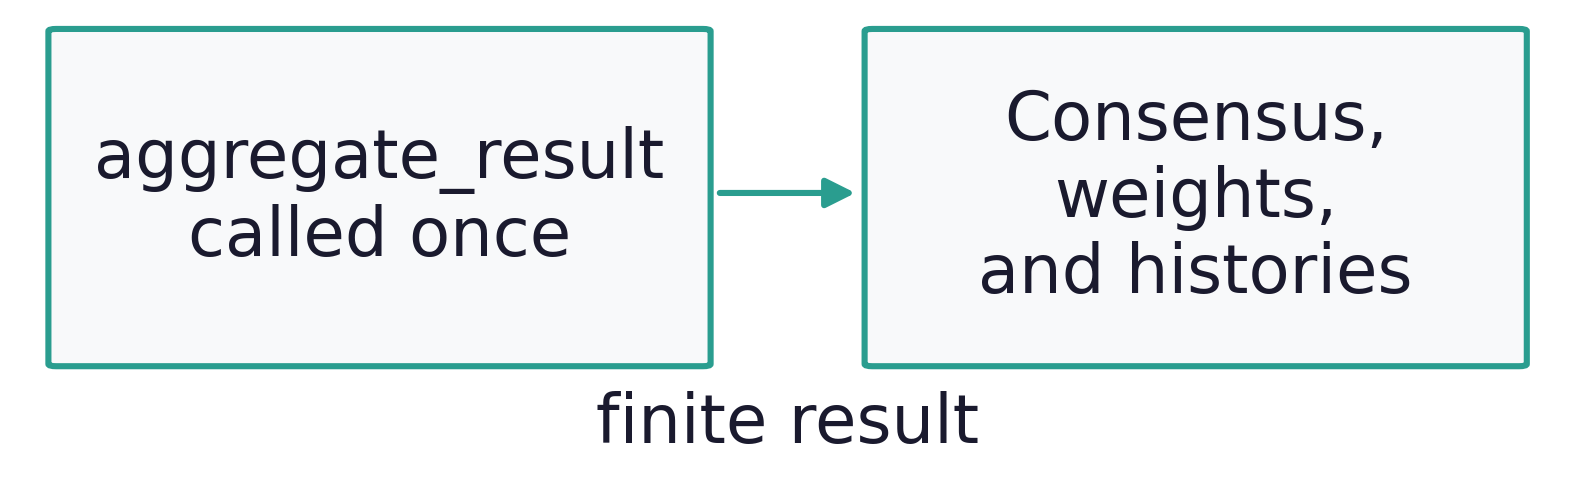
\includegraphics[keepaspectratio,width=0.98\linewidth,height=0.8\textheight,alt={aggregate\_result called once → Consensus, weights, and histories: finite result; data\_dependency.}]{../figures/application_integrity_flow.slide-aggregate-result-rich-result.png}
\refstepcounter{figure}\label{fig:application-integrity-flow-slide-panel-7}
\end{figure}
\end{frame}

\begin{frame}{Application integrity and\ldots{} (part 13)}
\begin{figure}
\centering
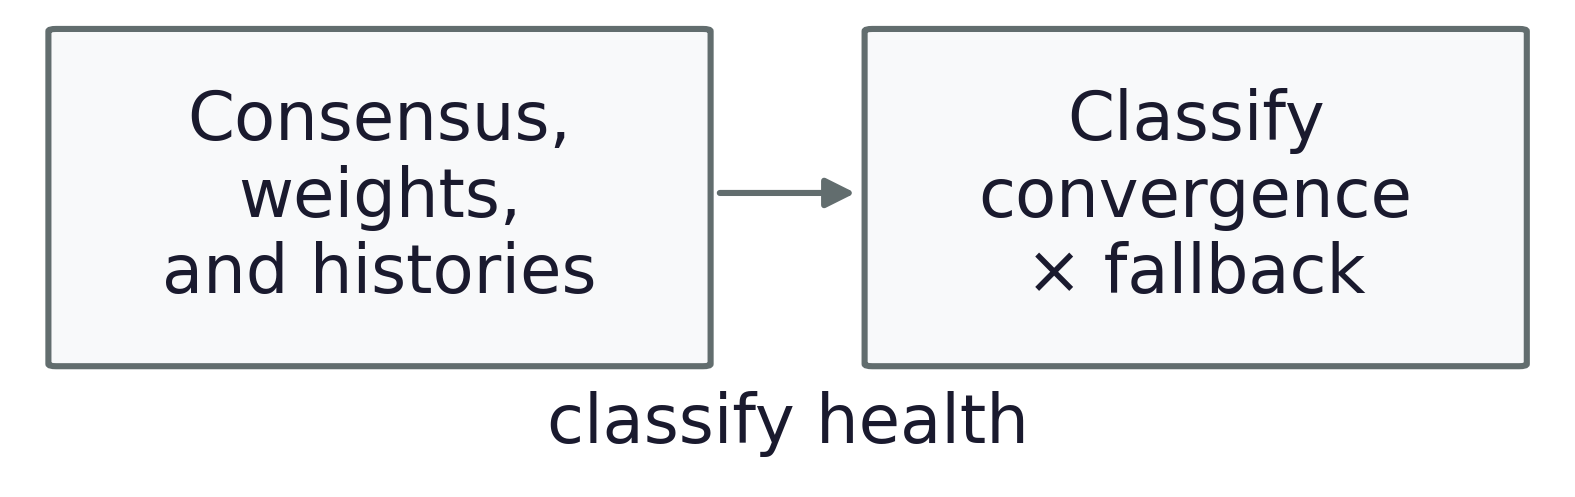
\includegraphics[keepaspectratio,width=0.98\linewidth,height=0.8\textheight,alt={Consensus, weights, and histories → Classify convergence × fallback: classify health; normal.}]{../figures/application_integrity_flow.slide-rich-result-solver-status.png}
\refstepcounter{figure}\label{fig:application-integrity-flow-slide-panel-8}
\end{figure}
\end{frame}

\begin{frame}{Application integrity and\ldots{} (part 14)}
\begin{figure}
\centering
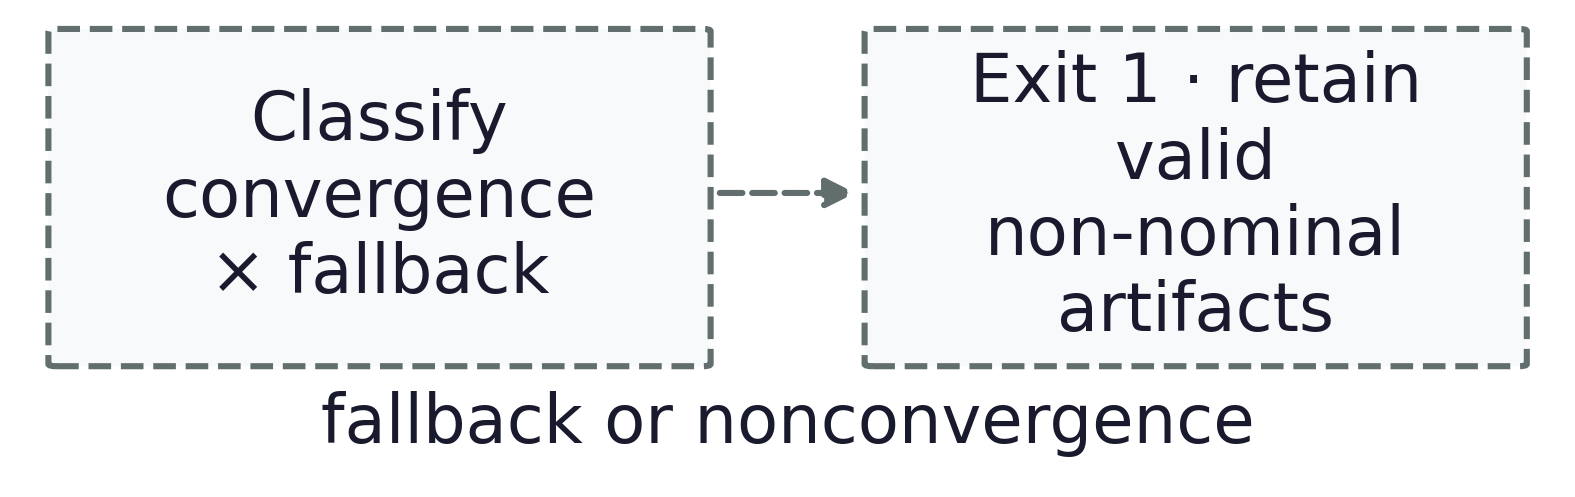
\includegraphics[keepaspectratio,width=0.98\linewidth,height=0.8\textheight,alt={Classify convergence × fallback → Exit 1 · retain valid non-nominal artifacts: fallback or nonconvergence; retained\_warning.}]{../figures/application_integrity_flow.slide-solver-status-non-nominal.png}
\refstepcounter{figure}\label{fig:application-integrity-flow-slide-panel-9}
\end{figure}
\end{frame}

\begin{frame}{Application integrity and\ldots{} (part 15)}
\begin{figure}
\centering

\includegraphics[keepaspectratio,width=0.98\linewidth,height=0.8\textheight,alt={Canonical request + SHA-256 → 1  request.json: semantic input; data\_dependency.}]{../figures/application_integrity_flow.slide-canonical-request-request-json.png}
\refstepcounter{figure}\label{fig:application-integrity-flow-slide-panel-10}
\end{figure}
\end{frame}

\begin{frame}{Application integrity and\ldots{} (part 16)}
\begin{figure}
\centering

\includegraphics[keepaspectratio,width=0.98\linewidth,height=0.8\textheight,alt={Consensus, weights, and histories → 2  result.json: semantic output; data\_dependency.}]{../figures/application_integrity_flow.slide-rich-result-result-json.png}
\refstepcounter{figure}\label{fig:application-integrity-flow-slide-panel-11}
\end{figure}
\end{frame}

\begin{frame}{Application integrity and\ldots{} (part 17)}
\begin{figure}
\centering
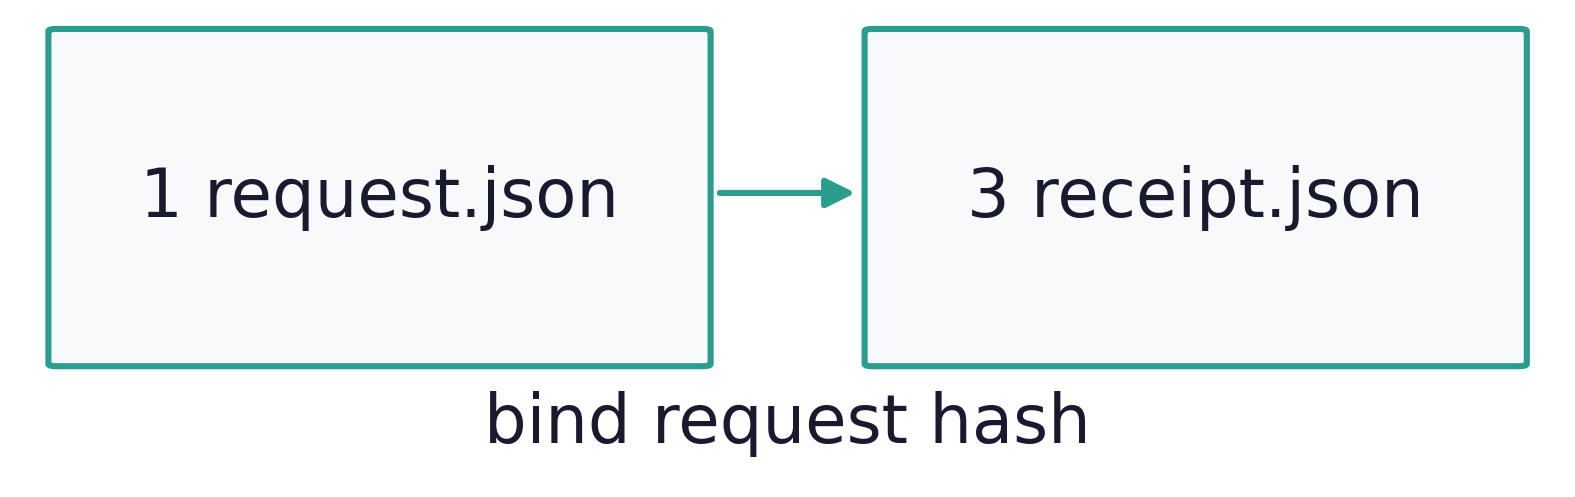
\includegraphics[keepaspectratio,width=0.98\linewidth,height=0.8\textheight,alt={1  request.json → 3  receipt.json: bind request hash; data\_dependency.}]{../figures/application_integrity_flow.slide-request-json-receipt-json.png}
\refstepcounter{figure}\label{fig:application-integrity-flow-slide-panel-12}
\end{figure}
\end{frame}

\begin{frame}{Application integrity and\ldots{} (part 18)}
\begin{figure}
\centering
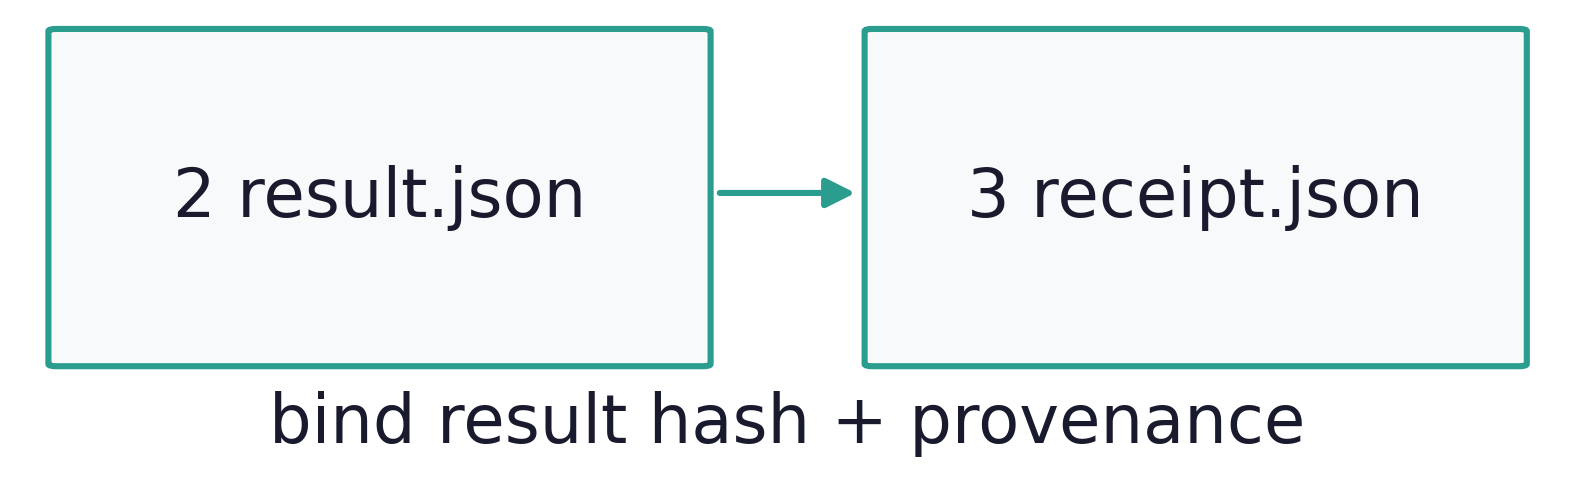
\includegraphics[keepaspectratio,width=0.98\linewidth,height=0.8\textheight,alt={2  result.json → 3  receipt.json: bind result hash + provenance; data\_dependency.}]{../figures/application_integrity_flow.slide-result-json-receipt-json.png}
\refstepcounter{figure}\label{fig:application-integrity-flow-slide-panel-13}
\end{figure}
\end{frame}

\begin{frame}{Application integrity and\ldots{} (part 19)}
\begin{figure}
\centering
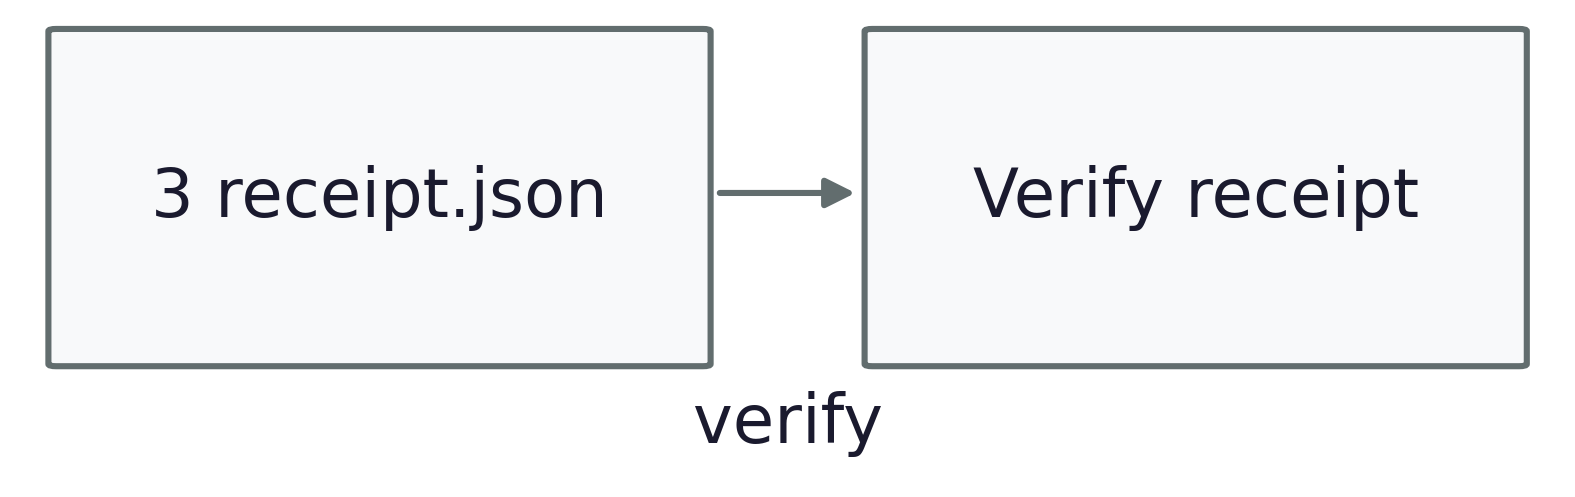
\includegraphics[keepaspectratio,width=0.98\linewidth,height=0.8\textheight,alt={3  receipt.json → Verify receipt: verify; normal.}]{../figures/application_integrity_flow.slide-receipt-json-verification.png}
\refstepcounter{figure}\label{fig:application-integrity-flow-slide-panel-14}
\end{figure}
\end{frame}

\begin{frame}{Application integrity and\ldots{} (part 20)}
\begin{figure}
\centering
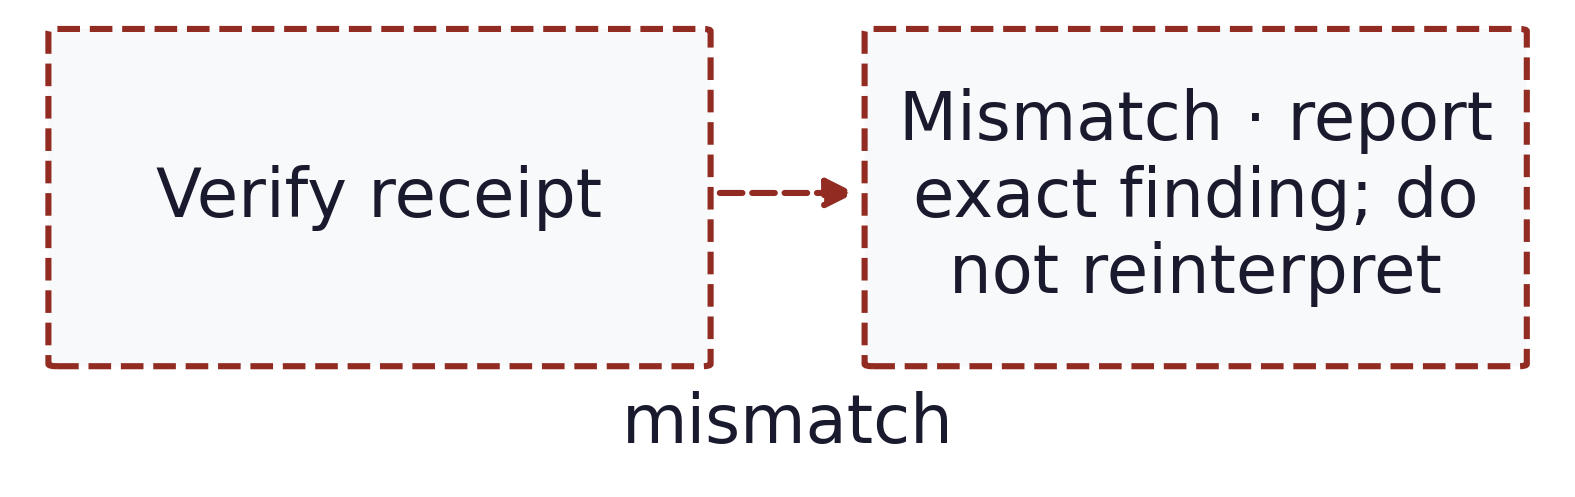
\includegraphics[keepaspectratio,width=0.98\linewidth,height=0.8\textheight,alt={Verify receipt → Mismatch · report exact finding; do not reinterpret: mismatch; rejected.}]{../figures/application_integrity_flow.slide-verification-mismatch.png}
\refstepcounter{figure}\label{fig:application-integrity-flow-slide-panel-15}
\end{figure}
\end{frame}

\begin{frame}{Application integrity and\ldots{} (part 21)}
\begin{figure}
\centering
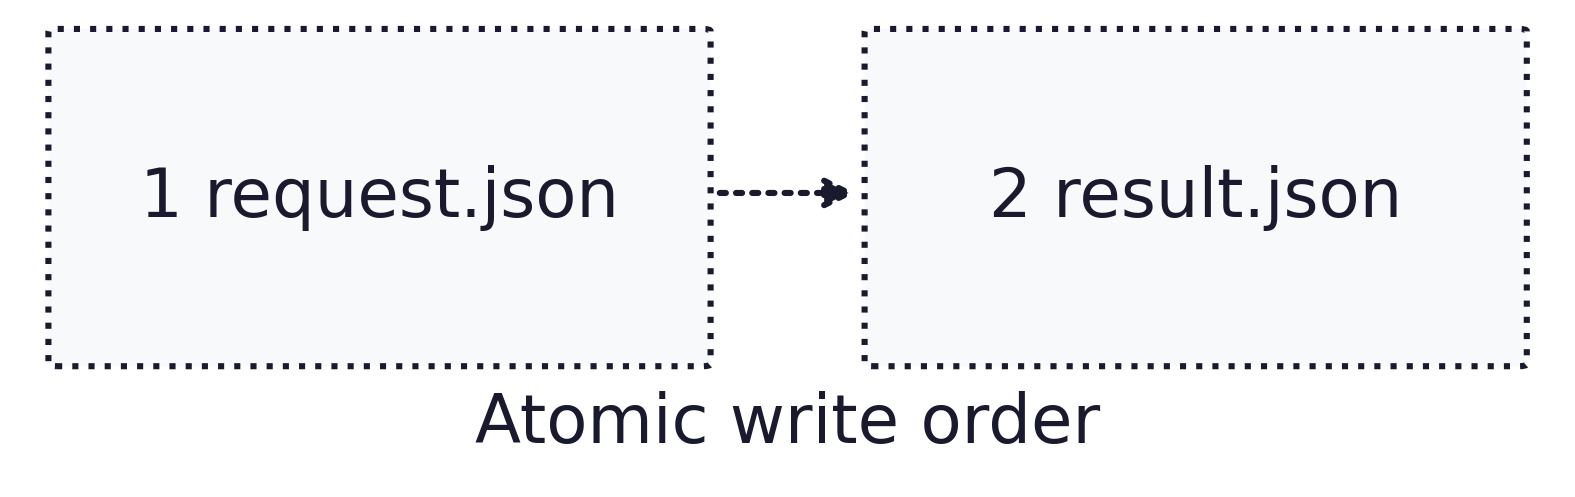
\includegraphics[keepaspectratio,width=0.98\linewidth,height=0.8\textheight,alt={1  request.json → 2  result.json: Atomic write order; write\_order.}]{../figures/application_integrity_flow.slide-write-request-json-result-json.png}
\refstepcounter{figure}\label{fig:application-integrity-flow-slide-panel-16}
\end{figure}
\end{frame}

\begin{frame}{Application integrity and\ldots{} (part 22)}
\begin{figure}
\centering
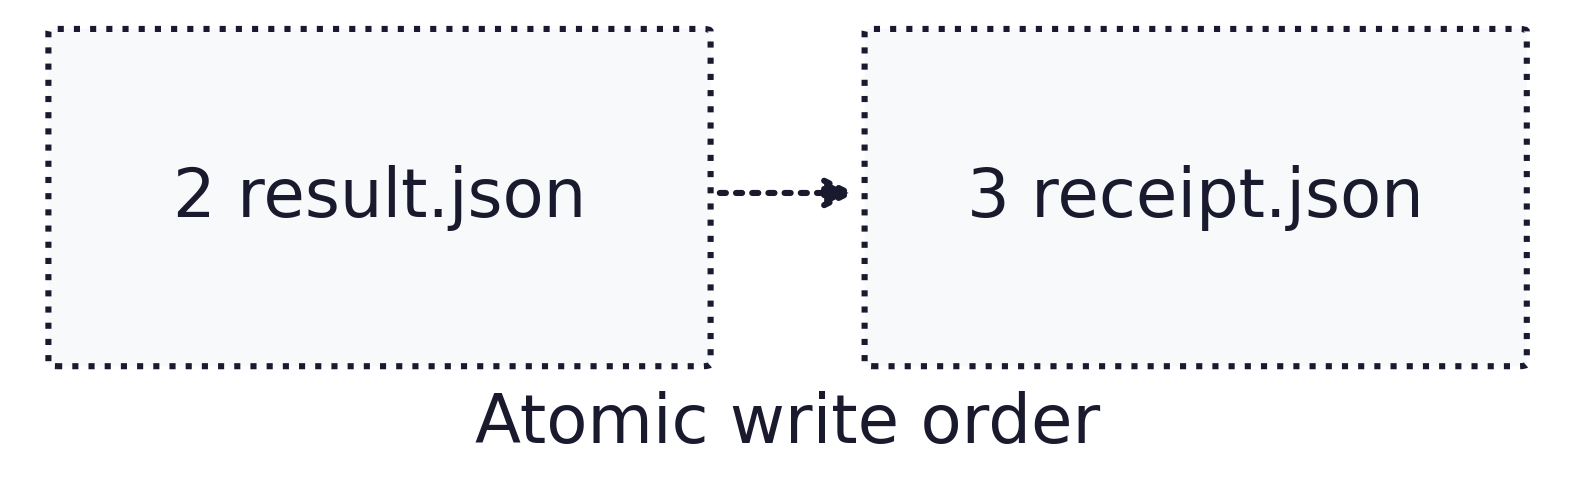
\includegraphics[keepaspectratio,width=0.98\linewidth,height=0.8\textheight,alt={2  result.json → 3  receipt.json: Atomic write order; write\_order.}]{../figures/application_integrity_flow.slide-write-result-json-receipt-json.png}
\refstepcounter{figure}\label{fig:application-integrity-flow-slide-panel-17}
\end{figure}
\end{frame}

\begin{frame}{Application integrity and\ldots{} (part 23)}
\begin{figure}
\centering

\includegraphics[keepaspectratio,width=0.98\linewidth,height=0.8\textheight,alt={converged · no fallback
nominal}]{../figures/application_integrity_flow.slide-status-nominal.png}
\refstepcounter{figure}\label{fig:application-integrity-flow-slide-panel-18}
\end{figure}
\end{frame}

\begin{frame}{Application integrity and\ldots{} (part 24)}
\begin{figure}
\centering

\includegraphics[keepaspectratio,width=0.98\linewidth,height=0.8\textheight,alt={converged · fallback
converged\_with\_fallback}]{../figures/application_integrity_flow.slide-status-converged-with-fallback.png}
\refstepcounter{figure}\label{fig:application-integrity-flow-slide-panel-19}
\end{figure}
\end{frame}

\begin{frame}{Application integrity and\ldots{} (part 25)}
\begin{figure}
\centering

\includegraphics[keepaspectratio,width=0.98\linewidth,height=0.8\textheight,alt={not converged · no fallback
not\_converged}]{../figures/application_integrity_flow.slide-status-not-converged.png}
\refstepcounter{figure}\label{fig:application-integrity-flow-slide-panel-20}
\end{figure}
\end{frame}

\begin{frame}{Application integrity and\ldots{} (part 26)}
\begin{figure}
\centering

\includegraphics[keepaspectratio,width=0.98\linewidth,height=0.8\textheight,alt={not converged · fallback
not\_converged\_with\_fallback}]{../figures/application_integrity_flow.slide-status-not-converged-with-fallback.png}
\refstepcounter{figure}\label{fig:application-integrity-flow-slide-panel-21}
\end{figure}
\end{frame}

\begin{frame}{Application integrity and\ldots{} (part 27)}
\begin{figure}
\centering

\includegraphics[keepaspectratio,width=0.98\linewidth,height=0.8\textheight,alt={Artifact integrity
Establishes: recorded request/result bytes match the receipt}]{../figures/application_integrity_flow.slide-artifact-integrity-establishes.png}
\refstepcounter{figure}\label{fig:application-integrity-flow-slide-panel-22}
\end{figure}
\end{frame}

\begin{frame}{Application integrity and\ldots{} (part 28)}
\begin{figure}
\centering

\includegraphics[keepaspectratio,width=0.98\linewidth,height=0.8\textheight,alt={Artifact integrity
Does not establish: equivalence to another source checkout or nominal solver health}]{../figures/application_integrity_flow.slide-artifact-integrity-does-not-establish.png}
\refstepcounter{figure}\label{fig:application-integrity-flow-slide-panel-23}
\end{figure}
\end{frame}

\begin{frame}{Application integrity and\ldots{} (part 29)}
\begin{figure}
\centering

\includegraphics[keepaspectratio,width=0.98\linewidth,height=0.8\textheight,alt={Source equivalence
Establishes: requested source inputs match recorded source provenance}]{../figures/application_integrity_flow.slide-source-equivalence-establishes.png}
\refstepcounter{figure}\label{fig:application-integrity-flow-slide-panel-24}
\end{figure}
\end{frame}

\begin{frame}{Application integrity and\ldots{} (part 30)}
\begin{figure}
\centering

\includegraphics[keepaspectratio,width=0.98\linewidth,height=0.8\textheight,alt={Source equivalence
Does not establish: calibration, domain suitability, or scientific validity}]{../figures/application_integrity_flow.slide-source-equivalence-does-not-establish.png}
\refstepcounter{figure}\label{fig:application-integrity-flow-slide-panel-25}
\end{figure}
\end{frame}

\begin{frame}{Application integrity and\ldots{} (part 31)}
\begin{figure}
\centering

\includegraphics[keepaspectratio,width=0.98\linewidth,height=0.8\textheight,alt={Nominal solver health
Establishes: the recorded run converged without fallback}]{../figures/application_integrity_flow.slide-nominal-solver-establishes.png}
\refstepcounter{figure}\label{fig:application-integrity-flow-slide-panel-26}
\end{figure}
\end{frame}

\begin{frame}{Application integrity and\ldots{} (part 32)}
\begin{figure}
\centering

\includegraphics[keepaspectratio,width=0.98\linewidth,height=0.8\textheight,alt={Nominal solver health
Does not establish: a downstream decision, acceptance, or truth of an interpretation}]{../figures/application_integrity_flow.slide-nominal-solver-does-not-establish.png}
\refstepcounter{figure}\label{fig:application-integrity-flow-slide-panel-27}
\end{figure}
\end{frame}

\begin{frame}{Application integrity and\ldots{} (part 33)}
\begin{figure}
\centering

\includegraphics[keepaspectratio,width=0.98\linewidth,height=0.8\textheight,alt={Application receipt does not establish:
calibration}]{../figures/application_integrity_flow.slide-no-claim-1.png}
\refstepcounter{figure}\label{fig:application-integrity-flow-slide-panel-28}
\end{figure}
\end{frame}

\begin{frame}{Application integrity and\ldots{} (part 34)}
\begin{figure}
\centering

\includegraphics[keepaspectratio,width=0.98\linewidth,height=0.8\textheight,alt={Application receipt does not establish:
domain suitability}]{../figures/application_integrity_flow.slide-no-claim-2.png}
\refstepcounter{figure}\label{fig:application-integrity-flow-slide-panel-29}
\end{figure}
\end{frame}

\begin{frame}{Application integrity and\ldots{} (part 35)}
\begin{figure}
\centering

\includegraphics[keepaspectratio,width=0.98\linewidth,height=0.8\textheight,alt={Application receipt does not establish:
scientific validity}]{../figures/application_integrity_flow.slide-no-claim-3.png}
\refstepcounter{figure}\label{fig:application-integrity-flow-slide-panel-30}
\end{figure}
\end{frame}

\begin{frame}{Application integrity and\ldots{} (part 36)}
\begin{figure}
\centering

\includegraphics[keepaspectratio,width=0.98\linewidth,height=0.8\textheight,alt={Application receipt does not establish:
downstream decision correctness}]{../figures/application_integrity_flow.slide-no-claim-4.png}
\refstepcounter{figure}\label{fig:application-integrity-flow-slide-panel-31}
\end{figure}
\end{frame}

\begin{frame}{Application integrity and\ldots{} (part 37)}
\begin{figure}
\centering

\includegraphics[keepaspectratio,width=0.98\linewidth,height=0.8\textheight,alt={Application receipt does not establish:
acceptance}]{../figures/application_integrity_flow.slide-no-claim-5.png}
\refstepcounter{figure}\label{fig:application-integrity-flow-slide-panel-32}
\end{figure}
\end{frame}

\begin{frame}{Environment fingerprint for the reported run}
\protect\phantomsection\label{sec:repro-environment}
The second reproduction input is the exact toolchain. Every field below
is captured by the successful full test-and-coverage receipt before
final variable generation rather than transcribed by hand.
\end{frame}

\begin{frame}{Environment fingerprint for\ldots{} (part 2)}
The receipt is bound to the source, tests, manuscript, source-owned
documentation, release metadata, ISC tree, dependency lock, and fresh
analysis receipt.
\end{frame}

\begin{frame}{Environment fingerprint for\ldots{} (part 3)}
It rejects any pre/post-suite drift in that boundary, so a reader
matching this environment and the seed above can reproduce the seeded
results; the config hash lets them confirm they are running the
configuration from which this manuscript was rendered.
\end{frame}

\begin{frame}{Environment fingerprint for\ldots{} (part 4)}
% template-accessible-table-inset
\begingroup
\setlength{\AFSlideTableWidth}{\textwidth}%
\setlength{\LTleft}{\fill}%
\setlength{\LTright}{\fill}%
\begin{longtable}[]{@{}
  >{\raggedright\arraybackslash}p{(\AFSlideTableWidth - 2\tabcolsep) * \real{0.4828}}
  >{\raggedright\arraybackslash}p{(\AFSlideTableWidth - 2\tabcolsep) * \real{0.5172}}@{}}
\label{tbl:repro_env}\tabularnewline
\toprule\noalign{}
\begin{minipage}[b]{\linewidth}\raggedright
Field
\end{minipage} & \begin{minipage}[b]{\linewidth}\raggedright
Value
\end{minipage} \\
\midrule\noalign{}
\endfirsthead
\toprule\noalign{}
\begin{minipage}[b]{\linewidth}\raggedright
Field
\end{minipage} & \begin{minipage}[b]{\linewidth}\raggedright
Value
\end{minipage} \\
\midrule\noalign{}
\endhead
Python & 3.12.12 \\
NumPy & 2.4.2 \\
SciPy & 1.18.0 \\
PyTorch (MLP complement) & 2.12.1 \\
\bottomrule\noalign{}
\end{longtable}
\endgroup
\end{frame}

\begin{frame}{Environment fingerprint for\ldots{} (part 5)}
The exact environment used for the reported run is recorded in
tbl.~11.
\end{frame}

\begin{frame}{Reader-surface accessibility boundary}
\protect\phantomsection\label{sec:repro-accessibility}
The validated HTML manuscript is the canonical accessibility-enhanced
reading surface. Its source gate requires a page language and title, a
skip link and main landmark, non-empty image alternatives, figure
captions, labelled full-size links, unique identifiers, resolved
references,
\end{frame}

\begin{frame}{Reader-surface\ldots{} (part 2)}
and present local assets on every generated page.
\end{frame}

\begin{frame}{Reader-surface\ldots{} (part 3)}
These deterministic checks are not a claim of WCAG conformance:
alternative-text quality, contrast, keyboard behavior, reading order,
reflow, mathematics, and assistive-technology behavior still require
manual review.
\end{frame}

\begin{frame}[fragile]{Reader-surface\ldots{} (part 4)}
The combined manuscript PDF is generated through the source-controlled
LuaLaTeX/tagpdf path and is released only when \texttt{pdfinfo} reports
\texttt{Tagged:\ yes}, qpdf exposes a non-empty \texttt{/Lang} and
\texttt{StructTreeRoot}, and the source-bound language check passes.
\end{frame}

\begin{frame}[fragile]{Reader-surface\ldots{} (part 5)}
Some Poppler builds omit the language line from \texttt{pdfinfo} even
when \texttt{/Lang} is present. The separate slide PDFs are checked
structurally, textually, through renderer logs during the producing run,
and by raster inspection, but do not inherit the manuscript tagging
status.
\end{frame}

\begin{frame}{Reader-surface\ldots{} (part 6)}
Renderer logs are retained with the external verification evidence
rather than the public source tree because they contain
environment-local timestamps and paths.
\end{frame}

\begin{frame}[fragile]{Reader-surface\ldots{} (part 7)}
Tagged structure is not PDF/UA conformance: a PDF/UA claim requires a
dedicated conformance report plus screen-reader and reading-order
review; \texttt{qpdf} structure checks and successful text extraction
alone are insufficient.
\end{frame}

\begin{frame}{Test and coverage evidence for the claim surface}
\protect\phantomsection\label{sec:repro-tests}
\textbf{Acceptance criteria.} 268 total, 266 passing.
\end{frame}

\begin{frame}{Test and coverage evidence\ldots{} (part 2)}
\textbf{Project test suite.} 2847 collected cases; the bound successful
receipt records zero failed cases. The project no-mocks policy remains a
separately executable source contract.
\end{frame}

\begin{frame}[fragile]{Test and coverage evidence\ldots{} (part 3)}
\textbf{Combined line and branch coverage on \texttt{src/}.} 90.57\%,
achieved by the bound full gate with branch measurement enabled. The
shared coverage threshold is \(\ge 90\%\) on this combined measure.
\end{frame}

\begin{frame}{Test and coverage evidence\ldots{} (part 4)}
To regenerate this evidence from a clean checkout, run the project suite
under the pinned development environment. Local execution and hosted CI
are separate results; the hosted checks must pass for the exact reviewed
commit before public integration. Both use the following coverage gate:
\end{frame}

\begin{frame}[fragile]{Test and coverage evidence\ldots{} (part 5)}
\texttt{uv} \texttt{run} \texttt{-\/-locked} \texttt{-\/-extra}
\texttt{dev} \texttt{pytest} \texttt{tests/}
\texttt{\textbackslash{}}\strut \\
\texttt{\ \ }\texttt{-\/-cov=src} \texttt{-\/-cov-fail-under=90}
\end{frame}

\begin{frame}{Test and coverage evidence\ldots{} (part 6)}
For a release-facing hydration, use the receipt-producing wrapper after
any required provisional pre-test render, then rerun hydration without
its provisional flag:
\end{frame}

\begin{frame}[fragile]{Test and coverage evidence\ldots{} (part 7)}
\texttt{uv} \texttt{run} \texttt{-\/-locked} \texttt{-\/-extra}
\texttt{dev} \texttt{python}
\texttt{scripts/validate\_test\_coverage.py}\strut \\
\texttt{uv} \texttt{run} \texttt{-\/-locked} \texttt{python}
\texttt{scripts/\textbackslash{}}\strut \\
\texttt{z\_generate\_manuscript\_variables.py}
\end{frame}

\begin{frame}{Artifact inventory for figures, data, and reports}
\protect\phantomsection\label{sec:repro-artifacts}
% template-accessible-table-inset
\begingroup
\setlength{\AFSlideTableWidth}{\textwidth}%
\setlength{\LTleft}{\fill}%
\setlength{\LTright}{\fill}%
\begin{longtable}[]{@{}
  >{\raggedright\arraybackslash}p{(\AFSlideTableWidth - 2\tabcolsep) * \real{0.5714}}
  >{\raggedright\arraybackslash}p{(\AFSlideTableWidth - 2\tabcolsep) * \real{0.4286}}@{}}
\label{tbl:repro_artifacts}\tabularnewline
\toprule\noalign{}
\begin{minipage}[b]{\linewidth}\raggedright
Category
\end{minipage} & \begin{minipage}[b]{\linewidth}\raggedright
Count
\end{minipage} \\
\midrule\noalign{}
\endfirsthead
\toprule\noalign{}
\begin{minipage}[b]{\linewidth}\raggedright
Category
\end{minipage} & \begin{minipage}[b]{\linewidth}\raggedright
Count
\end{minipage} \\
\midrule\noalign{}
\endhead
Figures & 1226 \\
Data files & 5 \\
Reports & 36 \\
\bottomrule\noalign{}
\end{longtable}
\endgroup
\end{frame}

\begin{frame}{Artifact inventory for\ldots{} (part 2)}
The top-level artifact counts in tbl.~12
complement the recursive, checksum-bearing release manifest.
\end{frame}

\end{document}
